% !TEX root = ../Диплом.tex

\section{Методы}

Данная секция описывает предложенные алгоритмы квадратизации и полиномиализации. Как для полиномиализации, так и для квадратизации будем рассматривать подходы с добавлением дифференциальных уравнений.

\subsection{Алгоритм полиномиализации} \label{poly-algo}

\subsubsection{Постановка задачи}

Дана система \ref{eq:1}. Найти минимальную полиномиализацию относительно числа введённых дополнительных уравнений.

Для начала перепишем подход из секции \ref{poly-diff} в более формальном виде. Как уже упоминалось в разделе \ref{AST-section}, нам удобно представлять правые части уравнений системы в виде абстрактных синтаксических деревьев. Из таких деревьев мы формируем лес, которые впоследствии мы будем анализировать.

\begin{algorithm}[H]
\SetAlgoLined
\SetKwFunction{FPoly}{Polynomialize}
\SetKwFunction{FGetNonPoly}{GetNonPolynomialItem}
\SetKwFunction{FFindNonPoly}{FindNonPolynomialItem}
\SetKwProg{Fn}{Function}{:}{}
\KwData{System - система вида \ref{eq:1}}
\KwResult{Полиномиализированная система}
\Fn{\FPoly{System}}{
    NewSystem = Копия(System)\;
    
    \tcc{Лес абстрактных синтаксических деревьев}
    Forest = \{\;\}
    
    \tcc{массив меток, где true - данное дерево не содержит неполиномиальных элементов}
    ForestIsPoly = \{\;\}
    
    \ForEach{r: правое уравнение системы}{
        tree = AST(r)\;
        Добавить(Forest, tree)\;
        ForestIsPoly[tree] = false\;
    }
    
    \While{ForestIsPoly содержит false}{
        g = \FGetNonPoly{Forest, ForestIsPoly}\;
        y_{new} = g\;
        \vec x = Переменные(NewSystem)\;
        ДобавитьУравнение(NewSystem, $\dot y_{new} = \frac{d\ g}{d \vec x} \dot {\vec x}$)\;
    }
    
    \Return NewSystem\;
}

\Fn{\FGetNonPoly{Forest, ForestIsPoly}}{
    \ForEach{tree: ForestIsPoly[tree] == false}{
        nonPolyItem = \FFindNonPoly{tree}\;
        \eIf{nonPolyItem $\ne$ null }{
            \Return nonPolyItem\;
        }{
            ForestIsPoly[tree] = true\;
        }
    }
    \Return null\;
}
\caption{Полиномиализация}
\end{algorithm}

\subsubsection{Прямой обход}

Разберём вариант реализации алгоритма FindNonPolynomialItem, который предполагает прямой проход по синтаксическому дереву - от корня к листьям.

\begin{algorithm}[H]
\SetAlgoLined
\SetKwFunction{FFindNonPoly}{FindNonPolynomialItem}
\SetKwProg{Fn}{Function}{:}{}
\KwData{node - узел AST, составленного из правой части уравнения системы \ref{eq:1}}
\KwResult{Неполиномиальный элемент или null, если такой не найдётся}

\Fn{\FFindNonPoly{node}}{
    \If{неПолиномиальнаяФункция(node)}{
        \Return node\;
    }
    
    \ForEach{child: дети node}{
        nonPolyItem = \FFindNonPoly{child}\;
        \If{nonPolyItem $\ne$ null}{
            \Return nonPolyItem\;
        }
    }
    \Return null\;
}

\caption{Прямой обход синтаксического дерева}
\end{algorithm}

\subsubsection{Обратный обход}

Теперь рассмотрим вариант реализации алгоритма FindNonPolynomialItem, который предпоагает обратный проход по синтаксическому дереву - от листьев к корню.

\begin{algorithm}[H]
\SetAlgoLined
\SetKwFunction{FFindNonPoly}{FindNonPolynomialItem}
\SetKwProg{Fn}{Function}{:}{}
\KwData{node - узел AST, составленного из правой части уравнения системы \ref{eq:1}}
\KwResult{Неполиномиальный элемент или null, если такой не найдётся}

\Fn{\FFindNonPoly{node}}{
    \ForEach{child: дети node}{
        nonPolyItem = \FFindNonPoly{child}\;
        \If{nonPolyItem $\ne$ null}{
            \Return nonPolyItem\;
        }
    }
    
    \If{неПолиномиальнаяФункция(node)}{
        \Return node\;
    }
    \Return null\;
}

\caption{Обратный обход синтаксического дерева}
\end{algorithm}

\subsubsection{Сравнение}

Разница в данных подходах заключается в том, как данные алгоритмы работают с композитным функциями $g = g_1 \circ g_2 \circ \cdots \circ g_k$. Прямой обход, наткнувшись на на неполиномиальную композитную функцию, возвращает сразу всё композицию. Обратный же подход, встретив такую функцию, вернёт максимально глубоко вложенный неполиномиальный элемент. 

Если мы рассматриваем полиномиализацию с введением алгебраических уравнений, то нам не столь важно, как сокращается композиция. Однако при подходе с введением дифференциальных уравнений нам приходится считать сложную производную найденного неполиномиального элемента. Вычислять сложные производные больших композиций дорого, поэтому мы постараемся этого избежать, предпочитая обратный обход прямому. 

\subsection{Алгоритм квадратизации} \label{quad-algo}

\subsubsection{Постановка задачи}

Как мы уже упоминали в разделе \ref{replacement-graph-section}, задача оптимальной квадратизации может быть сформулирована как задача поиска на графе замен. А именно, мы хотим найти квадратичную систему, представляющую собой узел графа замен, так, чтобы найденная квадратичная система находилась на минимальном расстоянии от узла исходной вершины.

Далее рассмотрим известные алгоритмы поиска, приведённые в разделе \ref{search-algo}, в контексте текущей задачи.

\subsubsection{BFS и DFS}

Поиск в глубину и поиск в ширину являются базовыми в задаче поиска, нередко оказываясь достаточно эффективными для многих задач. К сожалению, их в чистом виде достаточно применить для нашей задачи. Действительно, глубина всего графа замен может быть близка к бесконечной при неаккуратном выборе замен, что критично для DFS. В случае BFS нам мешает высокий коэффициент ветвления $b$, который, более того, растёт при для каждого последующего уровня глубины. Таким образом, BFS пригоден для практического использования только в том случае, когда искомая система находится на небольшой глубине. 

\subsubsection{DLS и ID-DLS}

В свете недостатоков BFS и DFS, весьма хорошо смотрится алгоритм поиска с ограничением глубины. Данный алгоритм не уходит дальше заданной глубины, что решает проблему DFS и просматривает узлы на желаемой глубине, а не последовательно идя по слоям, как BFS. Таким образом, при удачно выбранной конечной глубине и хорошем выборе замен на каждом шаге, мы сможем решать задачу за сравнительно небольшое число шагов.

Однако, если мы оценили конечную глубину ниже, чем глубину искомой вершины, то решить задачу мы не сможем. Решает эту проблему алгоритм ID-DFS, который представляет собой DLS, который увеличивает свою конечную глубину в том случае, если искомая вершина не найдена. Недостатком ID-DFS является необходмость исследовать граф заново, если на текущий шаг не нашёл нужную систему. Так же, увеличение глубины всегда происходит только на 1, что не всегда является оптимальной стратегией.

Поэтому мы несколько модифицируем ID-DFS, чтобы устранить данные недостатики. Введём новый алгоритм \textit{Поиск с ограничением глубины с итеративным углублением} (\textit{ID-DLS}), который отличается от ID-DFS в следующем:

\begin{enumerate}
    \item Вместо исследования графа заново после неудачной итерации, ID-DLS сохраняет вершины на текущей конечной глубине вместе с их исходящими заменами. В случае неудачного поиска мы сразу начинаем вычислять неисследованные элементы. Платой за это становится удвоенные затраты на память.
    \item Текущая конечная глубина более гибко изменяется за счёт функции $ОбновитьТекущуюКонечнуюГлубину$. Платой за это становится то, что гарантия оптимальности квадратизации ложится на приведённую функцию. Тем не менее, таким образом мы может искать суб-оптимальные решения с погрешностью, также определяемой функцией $ОбновитьТекущуюКонечнуюГлубину$.
\end{enumerate}

\begin{algorithm}[H]
\SetAlgoLined
\SetKwFunction{FIDDLS}{IDDLS}
\SetKwFunction{FDLS}{DLS}
\SetKwProg{Fn}{Function}{:}{}
\SetKwRepeat{Do}{do}{while}
\KwData{G - входной граф \\
v_{start} - входная вершина \\
prop - свойство, которым должна обладать выходная вершина \\
limit - финальная конечная глубина}
\KwResult{Вершина, обладающая свойством prop или null, если вершина не найдена}

 \Fn{\FIDDLS{G, v_{start}, prop, limit}}{
    currentLimit = 1\;
    
    \tcc{В данную очередь помещаются элементы на текущей конечной глубине вместе с их исходящими заменами. Фактически, мы лениво вычисляем вершины со следующего уровня}
    highDepthQueue = \{\ \}\;
    
    \Do{v == null}{
        \If{currentLimit > limit}{
            \Return null
        }
        v = \FDLS{G, v, prop, 1, currentLimit, highDepthQueue}\;
        currentLimit = ОбновитьТекущуюКонечнуюГлубину(currentLimit)\;
    }
    \Return v\;
 }
\caption{Поиск с ограничением глубины с итеративным углублением}
\label{algo:ID-DLS}
\end{algorithm}



\subsubsection{Выбор эвристик} \label{heuristics}

Точкой ветвления алгоритма квадратизация является шаг, на котором мы выбираем, в какой порядке исследовать возможные замены переменных. Таким образом, определим семейство эвристических функций в задаче квадратизации как 

\begin{equation}
    h:\ \mathbb{M} \longrightarrow \mathbb{R},
\end{equation}
где $\mathbb{M}$ - группа мономов, образованных над переменным $\vec x$ системы \ref{eq:1}. 

\begin{heuristics} \label{FF}
    \textit{Frequent-First}, \textit{FF} - эвристика, выбирающая моном, наиболее часто встречающийся в разложениях. Таким образом, замена переменной затронет наибольшее число мономов в системе.
    
    \begin{example}
        Для разложений $(x^2, xy), (xy, y^2, y^3, xy^2, xy^3), (x^2, y^2, xy)$ мы выберем моном $xy$, так как он встречается в трёх разложениях, а остальные не более чем в двух.
    \end{example}
\end{heuristics}

\begin{heuristics} \label{FVC}
    \textit{Free-Variables-Count}, \textit{FVC} - эвристика, выбирающая моном, образованный из наименьшего числа    переменых. Таким образом, в уравнении $y_i = m'(\vec x) \dot{\vec x}$, соответствующем данной замене, будет минимальное число слагаемых.
    
    \begin{example}
        Из мономов $x^2, xy, xyz$ мы выберем $x^2$, имеющий только одну переменную. Покажем ОДУ, образованные данными заменами:
        \begin{enumerate}
            \item $x^2 \longrightarrow \dot w = 2x \dot x$
            \item $xy \longrightarrow \dot w = \dot x y + x \dot y$
            \item $xyz \longrightarrow \dot w = \dot x yz + x \dot y z + xy \dot x$
        \end{enumerate}
    \end{example}
\end{heuristics}

\begin{heuristics} \label{AED}
    \textit{Auxiliary-Equation-Degree}, \textit{AED} - эвристика, выбирающая моном, порождающий уравнение с наименьшей степенью. 
    
    \begin{example}
        Пусть имеем систему со следующим респределение степеней: $degree(\dot x) = 1,\ degree(\dot y) = 2$. Тогда для замен $x^2, xy, y^2$ получим степени уравнений:
        \begin{enumerate}
            \item $x^2 \longrightarrow \dot w = 2x \dot x \longrightarrow 1 + 1 = 2$
            \item $xy \longrightarrow \dot w = \dot x y + x \dot y \longrightarrow max(1 + 1, 1 + 2) = 3$
            \item $y^2 \longrightarrow \dot w = 2y \dot y \longrightarrow 1 + 2 = 3$
        \end{enumerate}
        Из данных замен выберем $x^2$.
    \end{example}
\end{heuristics}

\begin{heuristics} \label{AEQD}
    \textit{Auxiliary-Equation-Quadratic-Discrepancy}, \textit{AEQD} - эвристика, выбирающая моном, чьё порождённое уравнение наименее отличается от квадратичного. Таким образом, замены, порождающие кважратичные уравнения, имеют самый высокий приоритет. 
    
    \begin{example}
        Пусть имеем замены, порождающие следующие уравнения
        \begin{enumerate}
            \item $m_1 \longrightarrow \dot w = x + y^2 + z^3 \longrightarrow 0 + 0 + 1 = 1$
            \item $m_2 \longrightarrow \dot w = x + y^2 + xy + z^3 \longrightarrow 0 + 0 + 0 + 1 = 1$
            \item $m_3 \longrightarrow \dot w = x + y^2 + z^3 + xyz \longrightarrow 0 + 0 +1 + 1 = 2$
        \end{enumerate}
        Таким образом, $m_1$ и $m_2$ имеют одинаковый приоритет, потому что порождённые ими уравнений имеют минимальную степерь 1.
    \end{example}
\end{heuristics}

\begin{heuristics} \label{AEQD}
    \textit{Summary-Monomial-Degree}, \textit{SMD} - эвристика, представляющая развитие идеи FF. Мы вибираем замену, которая максимально понижает степерь системы.
    
    \begin{example}
        Рассмотрим систему
        
        $\begin{array}{lcl}
             \dot x = xy^2 + y^3 \\
             \dot y = xy + x^2 y + 1
        \end{array}$
        \newline
        
        Понижение степени системы для замены $m$ вычисляетя как $N \cdot (degree(m) - 1)$, где $N$ - число мономов в системе, которые нацело делятся на $m$.
        \begin{enumerate}
            \item $y^2 \longrightarrow 2 \cdot (2 - 1) = 2$
            \item $xy \longrightarrow 3 \cdot (2 - 1) = 3$
            \item $y^3 \longrightarrow 1 \cdot (3 - 1) = 2$
        \end{enumerate}
        Получили, что замена $xy$ максимально сильно снижает степень системы.
    \end{example}
\end{heuristics}

\subsubsection{Правило параллелограмма}

Пусть для начальной полиномиальной системы $S$ имеются две замены $m_1$ и $m_2$.

\begin{wrapfigure}{R}{0.8\textwidth}
\begin{subfigure}{.4\textwidth}
  \centering
  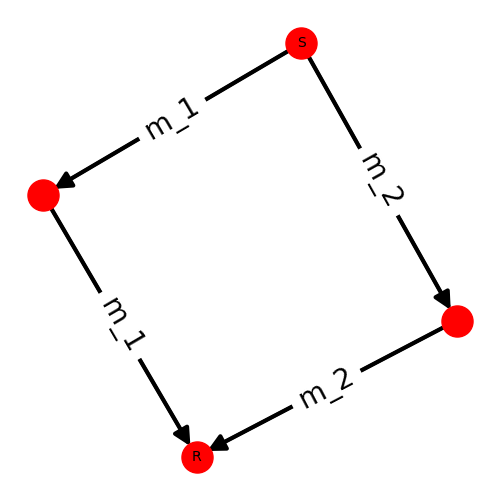
\includegraphics[width=0.8\linewidth]{chapters/images/parallel.png}  
  \caption{Граф замен для $S$}
  \label{fig:parallel-replacement-graph}
\end{subfigure}
\begin{subfigure}{.4\textwidth}
  \centering
  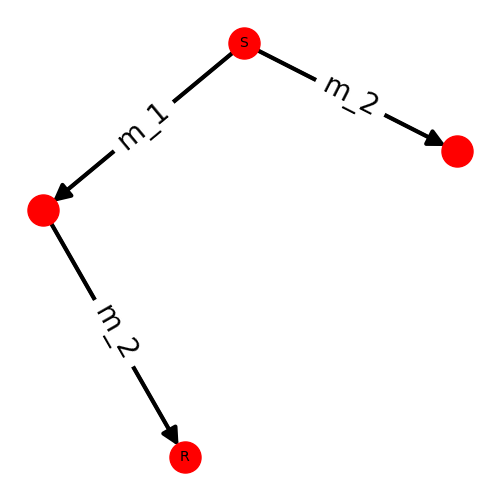
\includegraphics[width=0.8\linewidth]{chapters/images/parallel_red.png}  
  \caption{Упрощённый по правилу параллелограмма граф \ref{fig:parallel-replacement-graph}}
  \label{fig:parallel-replacement-graph-red}
\end{subfigure}
\caption{Правило параллелограмма}
\label{fig:parallel-rule}
\end{wrapfigure}

\begin{proposition}
    Замены $m_1$ и $m_2$ приведут к одной и той же системе $R$ вне зависимости от порядка их проведения. Действительно, ведь в таком случае введённые переменные $y_1$ и $y_2$ получаются перестановкой $[y_1 = y_2,\; y_2 = y_1]$.
\end{proposition}

Таким образом, мы можем убирать часть рёбер из графа во время его исследования. Данная оптимизация становится весьма важна для параллельных версий алгоритма, так как даёт возможность потокам оптимизировать работу друг друга.



